\section{初始点}
\label{sec:lpipm-initial-point}

上一节的计算从一个严格可行点出发。贯穿例的约束很简单，这样的点一眼可见，一般问题却未必。接下来要弄清：起点从哪里来，起点不可行时算法还能不能用，问题本身没有严格可行点时又该怎么办？

\paragraph{可行初始方法}
最直接的想法是先求出一个严格可行点，再开始路径跟踪，这和单纯形法的第一阶段是同一个思路。对原始一侧，构造辅助问题
\begin{equation}
 \min_{\bm{x},\rho}\ \rho\quad\text{s.t.}\quad\bm{A}\bm{x}=\bm{b},\quad\bm{x}+\rho\bm{1}\geq\bm{0},\quad\rho\geq-1.
 \label{eq:lpipm-phase-one}
\end{equation}
$\rho$越小，$\bm{x}$离边界越有余量。下界$-1$只是为了防止$\rho$在可行集无界时下降到负无穷。

这个辅助问题的严格可行点是现成的：任取$\bm{A}\bm{x}=\bm{b}$的一个解，例如最小范数解$\bm{A}^\top(\bm{A}\bm{A}^\top)^{-1}\bm{b}$，再取足够大的$\rho$即可。最优值$\rho^\star$的符号给出三种结论：

\begin{itemize}
 \item $\rho^\star<0$：最优点满足$x_i\geq-\rho^\star>0$，这是原问题的严格可行点。
 \item $\rho^\star=0$：原问题可行，但没有严格可行点。
 \item $\rho^\star>0$：原问题不可行。
\end{itemize}

三种情形可以用同一个小例子看到。取两个变量和约束$x_1+x_2=a$。把两个分量约束相加，得到$a+2\rho\geq0$，即$\rho\geq-a/2$。取$a=1$时，$\rho^\star=-1/2$，最优点$(1/2,1/2)$严格可行。取$a=0$时，$\rho^\star=0$，可行点只有原点。取$a=-1$时，$\rho^\star=1/2$，原问题不可行。

这个方法有两点不足。辅助问题本身也是线性规划，且它的对偶一侧未必有严格可行点：只有不存在非零的$\bm{d}\geq\bm{0}$使$\bm{A}\bm{d}=\bm{0}$时才有，否则要先加上足够大的变量上界。另外，对偶一侧还要另解一个类似的问题，求出来的点也通常离中心路径很远，要用$\sigma$接近$1$的几步先作中心化。这些原因使大规模实现很少走这条路。

\paragraph{不可行初始方法}
更常用的做法是放弃“起点满足等式”这个要求，只保持$\bm{x},\bm{s}>\bm{0}$。方程组~\eqref{eq:lpipm-newton}的右端本来就含$\bm{r}_{\mathrm{p}}$和$\bm{r}_{\mathrm{d}}$，上一节的公式可以原样使用。式~\eqref{eq:lpipm-residual-update}说明，每走步长$\alpha$，两个等式残差都精确地乘以$1-\alpha$。

这和可行初始方法的区别在于，等式约束不再是“先满足的前提”，而是和互补量一起逐步降低的目标。迭代点在走向最优的同时走向可行。

用贯穿例试算，起点取$\bm{x}^{(0)}=\bm{s}^{(0)}=\bm{1}$、$y^{(0)}=0$，它不满足任何等式。残差是
\[
 r_{\mathrm{p}}=2,\qquad\bm{r}_{\mathrm{d}}=(0,-1,-2)^\top,\qquad\mu^{(0)}=1.
\]
取$\sigma=0.3$，$\bm{r}_{\mathrm{c}}=-0.7\,\bm{1}$。

由式~\eqref{eq:lpipm-normal-data}，$\bm{D}=\bm{I}$，于是
\[
 M=3,\qquad h=-2-\sum_{i=1}^3\bigl(r_{\mathrm{c},i}+r_{\mathrm{d},i}\bigr)=3.1,\qquad\Delta y=\frac{31}{30}\approx1.0333.
\]
回代得到
\[
 \Delta\bm{s}\approx(-1.0333,-0.0333,0.9667)^\top,\qquad\Delta\bm{x}\approx(0.3333,-0.6667,-1.6667)^\top.
\]

$\alpha_{\max}=0.6$由$x_3$决定，取$\alpha=0.54$。新的残差恰好是原来的$0.46$倍，点是
\[
 \bm{x}^{(1)}=(1.18,0.64,0.10)^\top,\qquad y^{(1)}=0.558,\qquad\bm{s}^{(1)}=(0.442,0.982,1.522)^\top.
\]
可以核对$r_{\mathrm{p}}=1.92-1=0.92=0.46\times2$。

接下来第二轮取$\alpha\approx0.894$，第三轮取到$\alpha=1$，等式残差降到舍入误差水平，此后成为可行迭代，如图~\ref{fig:lpipm-infeasible-start}(a)。

\begin{BookInlineFigure}
  \centering
  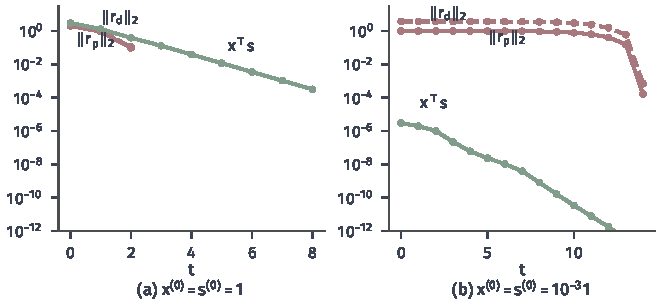
\includegraphics[width=112mm]{figures/05-optimization/01-linear-programming/matplotlib/lpipm-infeasible-start/figure.pdf}
  \caption{不可行起点的两种情况，贯穿例，$\sigma=0.3$、$\eta=0.9$，对数纵轴。红色实线是$\lVert\bm{r}_{\mathrm{p}}\rVert_2$，红色虚线是$\lVert\bm{r}_{\mathrm{d}}\rVert_2$，绿线是$\bm{x}^\top\bm{s}$。(a)起点$\bm{x}=\bm{s}=\bm{1}$，残差在第$3$轮取单位步后归零（图中不再画出）。(b)起点$\bm{x}=\bm{s}=10^{-3}\bm{1}$，互补量先极快地变小，而残差前十轮几乎不动，因为此间的步长只有$10^{-3}$到$10^{-1}$量级。}
  \label{fig:lpipm-infeasible-start}
\end{BookInlineFigure}

\paragraph{起点太小的后果}
图~\ref{fig:lpipm-infeasible-start}(b)把起点缩小到$10^{-3}\bm{1}$。这个起点的互补量已经小到$3\times10^{-6}$，等式残差却仍有$1$和$3.7$的量级。起点小，意味着方程$x_is_i\approx\sigma\mu$的线性化只允许很小的移动：Newton方向要消除大的等式残差，$\alpha_{\max}$却被很小的$x_i,s_i$限制，头几轮的步长只有约$7\times10^{-4}$。

算法最终还是走出来了，但这是这个例子的运气，不是一般保证。理论分析要求互补量不能比等式残差下降得快，常用的条件是
\begin{equation}
 \frac{\lVert(\bm{r}_{\mathrm{p}}^{(t)},\bm{r}_{\mathrm{d}}^{(t)})\rVert_2}{\mu^{(t)}}
 \leq C\,\frac{\lVert(\bm{r}_{\mathrm{p}}^{(0)},\bm{r}_{\mathrm{d}}^{(0)})\rVert_2}{\mu^{(0)}},
 \label{eq:lpipm-infeasible-ratio}
\end{equation}
其中$C\geq1$是常数，并且要求起点足够大。这种算法的全局收敛和复杂度结果需要较长的邻域分析，读者可查阅专著\scite{math-nocedal2006numerical}。在实现中，它对应的经验是起点的$\bm{x}$和$\bm{s}$要足够大，互补量相对残差不能太小。

\paragraph{一个常用的起点}
起点要兼顾两件事：接近满足等式，以及各分量足够大。一个常用的启发式分两步。先求最小范数意义下的近似：
\begin{equation}
 \tilde{\bm{x}}=\bm{A}^\top(\bm{A}\bm{A}^\top)^{-1}\bm{b},\qquad
 \tilde{\bm{y}}=(\bm{A}\bm{A}^\top)^{-1}\bm{A}\bm{c},\qquad
 \tilde{\bm{s}}=\bm{c}-\bm{A}^\top\tilde{\bm{y}}.
 \label{eq:lpipm-mehrotra-start}
\end{equation}
再把负分量和过小的分量整体平移成正的。贯穿例中$\bm{A}\bm{A}^\top=3$，于是$\tilde{\bm{x}}=\tfrac13\bm{1}$，$\tilde{y}=2$，$\tilde{\bm{s}}=(-1,0,1)^\top$。

平移分两步。第一步取$\delta_s=\max\{-1.5\min_i\tilde{s}_i,0\}=1.5$（$\tilde{\bm{x}}$已为正，$\delta_x=0$），得到$\hat{\bm{s}}=(0.5,1.5,2.5)^\top$。第二步按当前互补量再抬高一点，取
\[
 \hat{\delta}_x=\frac12\frac{\tilde{\bm{x}}^\top\hat{\bm{s}}}{\bm{1}^\top\hat{\bm{s}}}=\frac16,\qquad
 \hat{\delta}_s=\frac12\frac{\tilde{\bm{x}}^\top\hat{\bm{s}}}{\bm{1}^\top\tilde{\bm{x}}}=\frac34.
\]
最后的起点是
\[
 \bm{x}^{(0)}=\frac12\bm{1},\qquad y^{(0)}=2,\qquad\bm{s}^{(0)}=(1.25,2.25,3.25)^\top.
\]
这是一条经验规则，没有理论保证，但在实践中通常能避开图~\ref{fig:lpipm-infeasible-start}(b)的情形。

\paragraph{严格可行点不存在时}
定理~\ref{thm:lpipm-central-exists}说明，$\mathcal{F}^{\circ}$为空时中心路径不存在，路径跟踪失去了依据。这种情况有两类来源，处理方式不同。

一类来自建模的表述，问题本身可解。典型例子是把无符号变量写成两个非负变量之差$x=x^+-x^-$：两列互为相反数，第~\ref{sec:lpipm-central-path}节的反例已经说明，这样的问题对偶一侧没有严格可行点。又如约束$x_1+x_2=0$强迫两个变量恒为零。

\term{预处理}（presolve）承担这类任务：删去冗余的行以恢复满行秩，把被约束确定的变量代入，识别恒为零的变量，单独处理自由变量，并把行列缩放到相近的量级。预处理不改变最优解集（或给出恢复原解的办法），却能去掉一大批使严格可行性失效的结构。

另一类是问题真的不可行或无界。这时算法的迭代通常会发散，互补量和残差都下不去，但“没有收敛”不等于“证明了不可行”。我们需要一种方法，在问题不可解时也能输出一张可以核对的证书。

\paragraph{齐次自对偶嵌入}
思路是把原问题和对偶问题放进一个更大的、总有解的方程组里，用两个新的非负变量$\tau,\kappa$来判别结局。\term{齐次模型}（homogeneous model）是
\begin{equation}
 \begin{aligned}
 \bm{A}\bm{x}-\bm{b}\tau&=\bm{0},\\
 \bm{A}^\top\bm{y}+\bm{s}-\bm{c}\tau&=\bm{0},\\
 \bm{b}^\top\bm{y}-\bm{c}^\top\bm{x}-\kappa&=0,
 \end{aligned}
 \qquad\bm{x},\bm{s}\geq\bm{0},\quad\tau,\kappa\geq0.
 \label{eq:lpipm-homogeneous}
\end{equation}

零解总是满足它，所以这个模型不会没有解。不同的结局体现在非零解上：

\begin{itemize}
 \item $\tau>0$、$\kappa=0$：把$(\bm{x},\bm{y},\bm{s})$都除以$\tau$，前两行正是原始和对偶可行性，第三行说明目标相等，得到一对最优解。
 \item $\tau=0$、$\kappa>0$：此时$\bm{A}\bm{x}=\bm{0}$，$\bm{A}^\top\bm{y}+\bm{s}=\bm{0}$，且$\bm{b}^\top\bm{y}-\bm{c}^\top\bm{x}>0$，所以$\bm{b}^\top\bm{y}>0$或$\bm{c}^\top\bm{x}<0$至少有一个成立。
\end{itemize}

后一种情况给出的正是不可行证书。若$\bm{b}^\top\bm{y}>0$，则原问题不可行：假如有$\bar{\bm{x}}\geq\bm{0}$满足$\bm{A}\bar{\bm{x}}=\bm{b}$，由$\bm{A}^\top\bm{y}=-\bm{s}$，就有
\[
 \bm{b}^\top\bm{y}=\bar{\bm{x}}^\top\bm{A}^\top\bm{y}=-\bar{\bm{x}}^\top\bm{s}\leq0,
\]
与$\bm{b}^\top\bm{y}>0$矛盾。

若$\bm{c}^\top\bm{x}<0$，则对偶不可行：假如有$(\bar{\bm{y}},\bar{\bm{s}})$对偶可行，由$\bm{A}\bm{x}=\bm{0}$，就有
\[
 \bm{c}^\top\bm{x}=\bar{\bm{s}}^\top\bm{x}+\bar{\bm{y}}^\top\bm{A}\bm{x}=\bar{\bm{s}}^\top\bm{x}\geq0,
\]
与$\bm{c}^\top\bm{x}<0$矛盾。

用一个不可行的小问题走一遍：$\min x$，约束$x=-1$，$x\geq0$。这里$A=1$，$b=-1$，$c=1$，齐次模型是
\[
 x+\tau=0,\qquad y+s-\tau=0,\qquad -y-x-\kappa=0.
\]
第一式和非负性迫使$x=\tau=0$，第二式给出$s=-y$，第三式给出$\kappa=-y$。取$y=-1$，得到解$x=\tau=0$、$s=\kappa=1$。这时$\kappa>0$，$b\,y=1>0$，正是原问题不可行的证书。

齐次模型的理论要点是：模型的系数矩阵是斜对称的，并且存在严格互补解，其中$\tau$和$\kappa$恰有一个为正，所以结局一定是上面两种之一，原问题和对偶都不可行的情形归入后一种。式~\eqref{eq:lpipm-homogeneous}本身没有严格内点，实际的\term{齐次自对偶嵌入}（homogeneous self-dual embedding）再增加一个变量，构造出一个有明显严格内点、最优值为零的自对偶问题，于是路径跟踪可以从一个中心点直接开始。这一构造和收敛分析较长，读者可查阅专著的相关章节及其文献注记\scite{math-nocedal2006numerical}。

图~\ref{fig:lpipm-init-routes}总结了三条路线各自解决的问题。贯穿例和工厂问题都走中间这条路线或第一条路线即可；需要可靠地判别不可行、无界时，第三条路线是目前的标准选择。

\begin{BookInlineFigure}
  \centering
  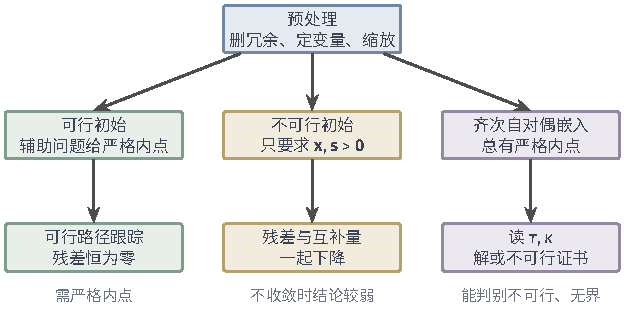
\includegraphics[width=105.738mm]{figures/05-optimization/01-linear-programming/tikz/lpipm-init-routes/figure.pdf}
  \caption{内点法起点的三条路线。预处理先去掉冗余和退化的结构。绿色路线先求严格可行点，迭代中残差恒为零；黄色路线只要求$\bm{x},\bm{s}>\bm{0}$，等式残差与互补量同时下降；紫色路线把问题嵌入一个总有严格内点的模型，由$\tau,\kappa$读出结局，并在问题不可解时给出证书。}
  \label{fig:lpipm-init-routes}
\end{BookInlineFigure}
